\subsection{UNet+++}
\subsubsection{Motivation}
After UNet and UNet++, we also try UNet+++\cite{unet_ppp},
which was developed and published in 2020 and maybe the latest UNet-like deep learning network.
In the following sections, we first briefly introduce UNet+++ according to the paper, and then introduce our training methods and results.

\subsubsection{Network description}
In image segmentation, Combining multi-scale features is one of important factors for accurate segmentation.
In recent deep learning network like UNet and UNet++, feature maps in different scale explore distinctive information. Lowlevel detailed feature maps capture rich spatial information, 
while high-level semantic feature maps embody position information. 
Nevertheless, these exquisite signals may be gradually diluted when progressively down- and up-sampling.
However, by implementing full-scale skip connections, UNet+++ can make full use of the multi-scale features, incorporating low-level details with high-level semantics from feature maps in different scales. 
Figure./ref{fig:unetpppGraph} shows simplified overviews of UNet+++. The image is from \cite{unet_ppp}.

\begin{figure}[!htpb]
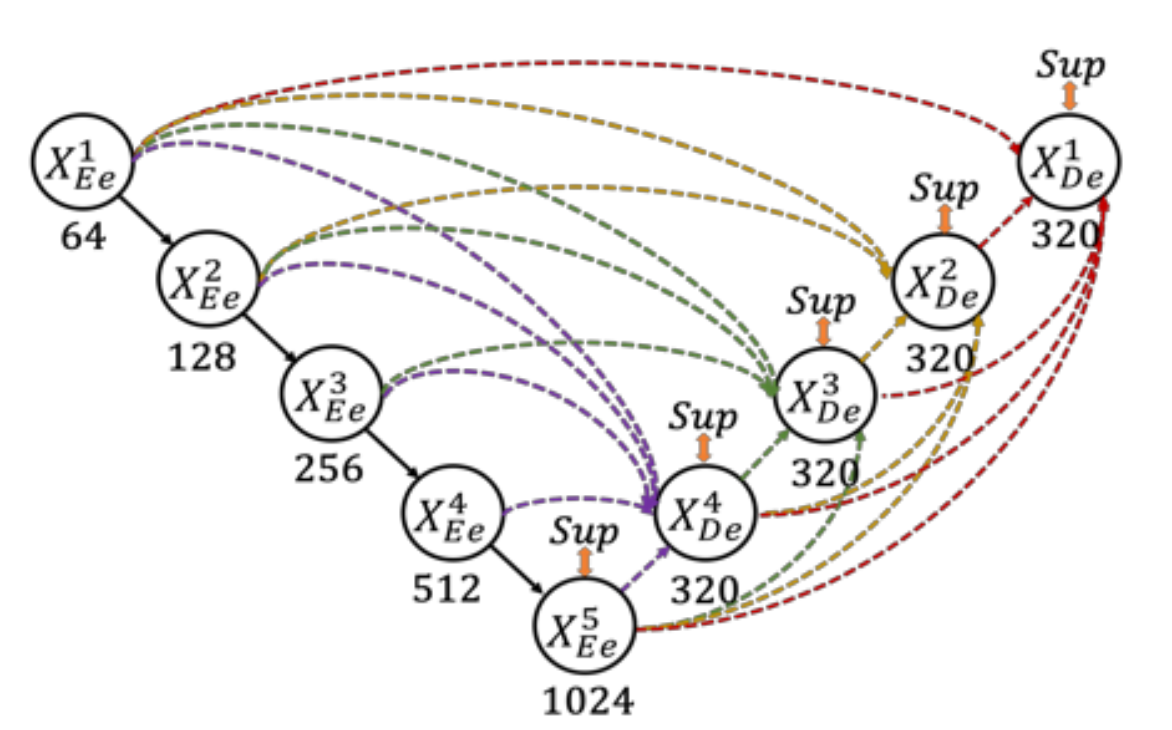
\includegraphics[width=\linewidth]{figuras/unet3+.png}
\caption{UNet+++ network structure}
\label{fig:unetpppGraph}
\end{figure}